\lecture[2022-05-17]{Data Sampling and Probability}
Previously, we mentioned the \href{fig:ds-lifecycle}{data science lifecycle}. Today, we focus on step 2: collecting data. How do we collect data?
\begin{center}
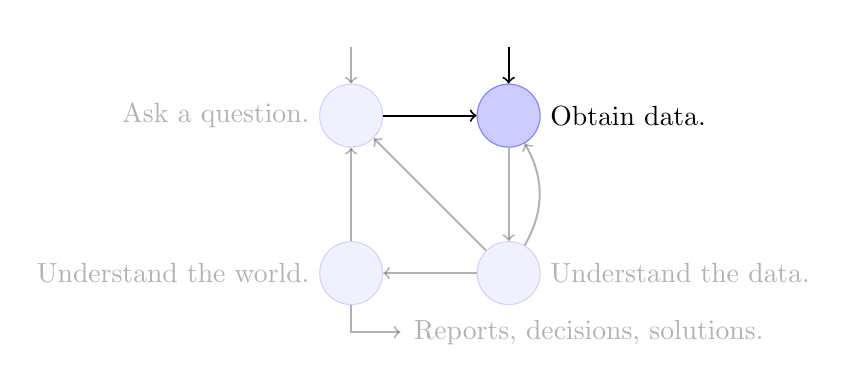
\begin{tikzpicture}
\node (aup) at (-1, 2) [draw=none] {};
\node (dup) at (1, 2) [draw=none] {}; 
\node (result) at (-0.25, -1.75) [draw=none, minimum size=0mm, label={[xshift=-2mm, opacity=0.3]right:Reports, decisions, solutions.}, opacity=0.3] {};
\node (ask) at (-1, 1) [circle, draw=blue!50, fill=blue!20, minimum size=8mm, label={[opacity=0.3]left:Ask a question.}, opacity=0.3] {};
\node (data) at (1, 1) [circle, draw=blue!50, fill=blue!20, minimum size=8mm, label=right:Obtain data.] {};
\node (uworld) at (-1, -1) [circle, draw=blue!50, fill=blue!20, minimum size=8mm, label={[opacity=0.3]left:Understand the world.}, opacity=0.3] {};
\node (udata) at (1, -1) [circle, draw=blue!50, fill=blue!20, minimum size=8mm, label={[opacity=0.3]right:Understand the data.}, opacity=0.3] {};
\draw [->, line width=0.25mm, opacity=0.3] (aup) edge (ask) (data) edge (udata) (udata) edge (uworld) (uworld) edge (ask) (udata) edge (ask);
\draw [->, line width=0.25mm] (dup) edge (data) (ask) edge (data);
\draw [->, bend right, line width=0.25mm, opacity=0.3] (udata) edge (data);
\draw [->, to path = (\tikztostart) |- (\tikztotarget), line width=0.25mm, opacity=0.3] (uworld) edge (result);
\end{tikzpicture}
\end{center}

\subsection{Sampling}

\subsubsection{Censuses and Surveys}
US decennial census - last held in April 2020. Counts \textit{every person} living in all 50 states, DC, and US territories - not just citizens. Mandated by the constitution and participation is required by law.

Important uses of the census:
\begin{itemize}
\item Allocation of federal funds.
\item Congressional representation (update based on population).
\item Drawing congressional/state representative districts.
\end{itemize}

\begin{definition}[Census]{In general, a census is an official count or survey of a population, typically recording various details of individuals.
}
\end{definition}

\begin{definition}[Survey]{A survey is a set of questions; e.g. workers survey individuals and households.

What and how the questions are asked can affect how the respondent answers or whether they answer at all.
}
\end{definition}

\subsubsection{Sampling: Definitions}
While a census is great, it is expensive and difficult to execute (e.g. would all voters be willing to participate in a voting census before an election?). For this, we can use samples.

\begin{definition}[Sample]{A sample is a subset of the population.
\begin{itemize}
\item Often used to make inferences about the population.
\item How the sample is drawn will affect its accuracy.
\item Common sources of error:
\begin{itemize}
\item \textbf{Chance error}: random samples vary from what is expected in any direction.
\item \textbf{Bias}: systematic error in one direction.
\end{itemize}
\end{itemize}
}
\end{definition}
\textbf{Population, Sample, and Sampling Frame}
\begin{itemize}
\item \textbf{Population}: group you want to learn something about.
\item \textbf{Sampling Frame}: list from which the sample is drawn (e.g. if you are sampling people, the sampling frame is the set of all people who can end up in the sample).
\item \textbf{Sample}: who you actually end up sampling; a subset of the sampling frame.
\end{itemize}
\begin{figure}[ht]
\begin{center}
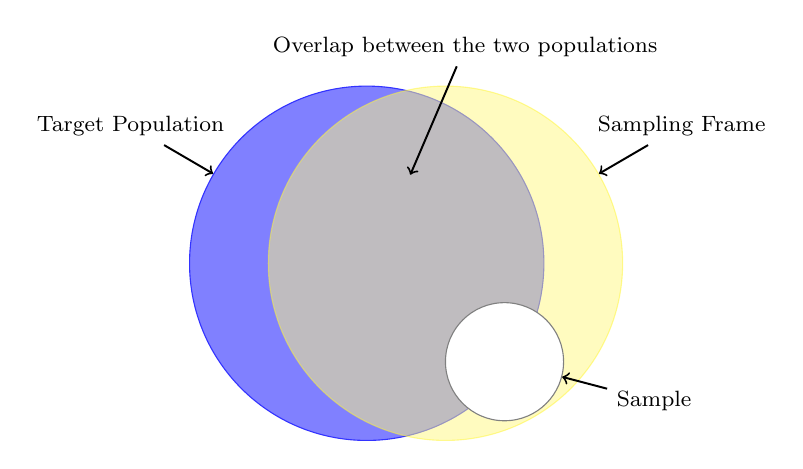
\begin{tikzpicture}
\node[circle, draw=blue!80, fill=blue!50, minimum size=45mm] (target) at (-0.5,0) {};
\node[circle, draw=yellow!80, fill=yellow!50, minimum size=45mm, opacity=0.5] (sframe) at (0.5, 0) {};
\node[circle, draw=black!50, fill=white, minimum size=15mm] (sample) at (1.25, -1.25) {};
\node[draw=none] (ol) at (0.75, 2.75) {\footnotesize Overlap between the two populations};
\node[draw=none] (tp) at (-3.5, 1.75) {\footnotesize Target Population};
\node[draw=none] (sf2) at (3.5, 1.75) {\footnotesize Sampling Frame};
\node[draw=none] (s2) at (3.15, -1.75) {\footnotesize Sample};
\node[draw=none] (dummy) at (0, 1) {};
\draw[->, line width=0.25mm] (sf2) edge (sframe) (s2) edge (sample) (tp) edge (target) (ol) edge (dummy);
\end{tikzpicture}
\end{center}
\caption{Target Population, Sampling Frame, and Sample. Note that there may be people in the sampling frame (and therefore, the sample) which are not part of the population.}
\end{figure}

\subsubsection{Bias: A Case Study}
\textbf{1936 Presidential Election}

Here, President FDR went up for re-election against Alf Landon. Polls were conducted in the months leading up to the election trying to predict the outcome.

One of the polls was from The Literary Digest, a magazine which had successfully predicted the outcome of 5 general elections up till 1936. Their survey was sent to 10 million people from phone books, magazines subscribers, and country club members. This poll got that 43\% of people would choose FDR in the election, but in the actual election, 61\% of people chose FDR.

\textbf{Literary Digest poll: What went wrong?}
\begin{enumerate}
\item Sampling frame was not representative of the US population.
\begin{itemize}
\item Chose people who had phone numbers and subscribed to their magazines or country clubs. 
\item Such people tend to be more affluent and more likely to vote Republican.
\end{itemize}
\item Non-response: only 2.4 million people (24\%) filled out the survey. Who knows how the other 76\% would have responded?
\end{enumerate}

\textbf{Gallup's Poll}

In addition to the Literary Digest poll, George Gallup also made predictions about the 1936 elections. Looking at the table, his result (56\%) was much closer to the actual election and with a smaller sample size.
\begin{center}
\begin{tabular}{@{}lll@{}}
\toprule
     & \% Roosevelt & \# surveyed \\
\midrule
    Election & 61\% & All voters ($\sim$45 million) \\
    Literary Digest Poll & 43\% & 10 million \\
    Gallup's Poll & 56\% & 50 000 \\
    Gallup's prediction of Digest's Poll & 44\% & 3 000 \\
\bottomrule
\end{tabular}
\end{center}
Gallup was even able to predict the Literary Digest's prediction within 1\% using a much smaller sample size. Why?
\begin{itemize}
\item He predicted their sampling frame (phonebook, magazine subscribers, country clubs).
\item So he sampled the same individuals.
\end{itemize}

\textbf{Common Biases}

Samples, while convenient, are subject to chance error and bias.
\begin{itemize}
\item \textbf{Selection Bias}: Systematically avoiding/favoring particular groups. Avoid by examining the sampling frame and the method of sampling.
\item \textbf{Response Bias}: People don't always respond truthfully. Avoid by examining the nature of questions and the method of surveying.
\item \textbf{Non-response Bias}: People don't always respond. Avoid by making surveys short and being persistent - people who don't respond aren't like the people who do.
\end{itemize}
It's likely that the Literary Digest sample was a case of selection bias - they favored choosing those who they could easily access through the phonebook/subscriptions.

\subsection{Probability}
\subsubsection{Probability Samples}
When sampling, go for quality over quantity - don't just go for a big sample (as that can lead to having a big sample that is of poor quality).

\textbf{Common Non-Random Samples}
\begin{itemize}
\item \textbf{Convenience Sample}: choose whoever you can get ahold of (e.g. when trying to measure the weight of mice, choosing whichever mice you can get ahold of as samples to measure weight).
\begin{itemize}
\item Not a good idea for inference.
\item Haphazard $\neq$ random.
\item Sources of bias can be present in ways that you may not think of (e.g. all the convenient samples can be of one group).
\end{itemize}
\item \textbf{Quota Sample}: Specify desired breakdown of various subgroups in population, then choose to reach targets however you can (e.g. Sampling individuals in your town and having the sample match the age distribution from the census).
\begin{itemize}
\item Reaching quotas ``however you can'' is not random.
\item Sample will represent some of the population (e.g. age), but not all of the population (e.g. gender, ethnicity, income may not be well represented in the sample).
\end{itemize}
\end{itemize}
So why sample at random? One thing is to reduce bias (despite this, random samples can still produce biased estimates); however, the main reason is that we can estimate bias and chance error with random samples, allowing us to quantify uncertainty.
\begin{definition}[Probability Sample]{Sample from a random sampling scheme. Has the following properties:
\begin{itemize}
\item Must be able to provide the chance that any specified set of individuals will be in the sample.
\item All individuals in the population need not have the same chance of being selected.
\item Will be able to measure the errors since you know all the probabilities.
\end{itemize}
}
\end{definition}
\begin{example}[]{Suppose there are 3 students: A, B, and D. Sample 2 students with the following procedure:
\begin{itemize}
\item Choose A with probability 1.
\item Choose from $\{B,D\}$ with probability 0.5 each.
\end{itemize}
\textbf{Possible Outcomes:}
\begin{center}
\begin{tabular}{@{}cc@{}}
\toprule
    Subsets of 2 & Probabilities \\
\midrule
    $\{A,B\}$ & 0.5 \\
    $\{A,D\}$ & 0.5 \\
    $\{B,D\}$ & 0 \\
\bottomrule
\end{tabular}
\end{center}
This is a probability sample, though not a great one:
\begin{itemize}
\item Of the 3 people in each population, know the probability (chance) of getting each subset.
\item If we're measuring the average distance students live from campus, then problems arise:
\begin{itemize}
\item The sampling frame does not account for the entire population - only three students.
\item Some \textit{chance error} depending on if the sample is AB or AD.
\item Since we choose A w.p. 1, the sample \textit{biases} towards A's response
\end{itemize}
\end{itemize}
}
\end{example}
\textbf{Common Random Sample Schemes}
\begin{itemize}
\item \textbf{Random Sample with replacement}: sample drawn uniformly at random with replacement.
\item \textbf{Simple random sample (SRS)}: sample drawn uniformly at random without replacement.
\begin{itemize}
\item Each individual/subset of individuals has the same chance of being selected.
\item Each pair has the same chance as every other pair; each triple has the same chance as every other triple (independent).
\end{itemize}
\end{itemize}
\begin{notebox}[]
Random doesn't always mean ``uniformly at random'', but with these examples, it does.
\end{notebox}
\begin{example}[]{Consider the following sampling scheme:
\begin{itemize}
\item Class roster has 1100 students listed alphabetically.
\item Pick one of first 10 students on the list at random.
\item Given the number from previously, sample the student and every 10th student listed after that (e.g. students 8, 18, 28, ...).
\end{itemize}
Determine the following:
\begin{enumerate}
\item Is this a probability sample?
\item Does each student have the same probability of being selected?
\item Is this a simple random sample?
\end{enumerate}
\tcbline
\begin{enumerate}
\item Yes, we can provide the probability of each subset being elected, e.g. $\Pr(S=\{8, 17, \ldots\}) = 0$, $\Pr(S=\{8, 18, \ldots\}) = \frac{1}{10}$.
\item Yes, each student has a 1/10 chance of being selected.
\item No, the samples are not independent - the probabilities are different for each pair. As noted above, $\Pr(\{8, 17\} \in S) = 0 \neq \Pr(\{8, 18\} \in S) = \frac{1}{10}$.
\end{enumerate}
}
\end{example}
Often, in data science, the population is large, but we can only afford to sample a small number of individuals. If the population is relatvely large compard to the sample, then sampling with and without replacement are pretty much the same.
\begin{example}[Sampling with/without Replacement]{Suppose there are 10 000 people in the population; 7 500 who like Snack 1 and 2 500 who like Snack 2. Find the probability of all people in a sample of 20 liking Snack 1 with and without replacement.
\tcbline 
\begin{itemize}
\item \textbf{SRS/Without Replacement}: first probability is $\frac{\text{\# people who like S1}}{\text{Population}}$, then $\frac{\text{\# people who like S1}-i+1}{\text{Population}-i+1}$ for the $i$th person.
\[
P(\text{All 20 people like S1}) = \left(\frac{7500}{1000}\right) \left(\frac{7499}{9999}\right) \cdots \left(\frac{7482}{9982}\right) \left(\frac{7481}{9981}\right) \approx 0.03153   
.\] 
\item \textbf{With Replacement}: all probabilities are $\frac{\text{\# people who like S1}}{\text{Population}} = \frac{3}{4}$.
\[
P(\text{All 20 people like S1}) = \left(\frac{3}{4}\right)^{20} \approx 0.003171
.\] 
\end{itemize}
The results are close as the without replacement proportion remains close to the with replacement proportion; however, it is easier to calculate the probability without replacement.
}
\end{example}
\textbf{Recap}

If a sample was randomly sampled with replacement from a population:
\begin{itemize}
\item It is a probability sample.
\item We can quantify error and bias.
\item Given the population distribution, we can compute the probability of getting a particular sample.
\end{itemize}
\begin{notebox}[]
We almost never know the population distribution unless we take a census. However, framing allows us to quantify our uncertainty in any analysis/inference using our sample.
\end{notebox}

\begin{example}[Application: The Gallup Poll Today]{tbc
}
\end{example}

\subsubsection{Multinomial and Binomial Probabilities}
Binomial and multinomial probabilities arise when we: 
\begin{itemize}
\item Sample at random with replacement. (Think of as same trial)
\item Sample a fixed number (n) times.
\item Sample from a categorical distribution: 2 - binomial, $>2$ - multinomial.
\begin{center}
\begin{tabular}{@{}lll@{}}
\toprule
    & Binomial & Multinomial \\
\midrule
    \# Categories & 2 categories & $>2$ categories \\
    Example & Bag of Marbles: 60\% blue, 40\% not blue & Bag of Marbles: 60\% blue, 30\% green, 10\% red \\
\bottomrule
\end{tabular}
\end{center}
\end{itemize}
\textbf{Goal}: count the number in each category that end up in our sample. \mintinline{text}{np.random.multinomial} returns these counts.

\begin{example}[Binomial Probability]{Suppose we sample at random with replacement 7 times from a bag of marbles (60\% blue - b, 40\% not blue - n). Define the following events:
\begin{itemize}
\item A: Get the following marbles in the following order: bnbbbnn.
\item B: Get 4 blue marbles and 3 not blue marbles.
\end{itemize}
Find $\Pr(A)$. Is $\Pr(B)$ greater than, the same as, or smaller than $\Pr(A)$?
\tcbline 
\begin{align*}
    \Pr(A) &= (0.6) \cdot (0.4) \cdot (0.6)^3 \cdot (0.4)^2 \\
    &= (0.6)^4(0.4)^3
.\end{align*}
$\Pr(B) > \Pr(A)$. This is since A is a specific case of B (4 blues, 3 not blues). B could have any permutation of the marbles as long as there are 4 blue marbles out of 7. Therefore, there are more outcomes under event B, and since each outcome is uniform, the probability of B (multiple outcomes) happening is greater than A (one outcome).
\[
\Pr(B) = \left( \frac{7!}{4!3!} \right) (0.6)^4 (0.4)^3 = \binom{7}{4} (0.6)^4 (0.4)^3
.\]
}
\end{example}

\begin{example}[Multinomial Probability]{Sample with replacement 7 times from a bag of marbles (60\% blue, 30\% green, 10\% red). Define the following events:
\begin{itemize}
\item A: Get the following marbles in the following order: bgbbbgr.
\item B: Get 4 blue marbles, 2 green marbles, and 1 red marble.
\end{itemize}
\tcbline 
To find A, use the product rule for independent marble draws:
\begin{align*}
    \Pr(A) &= (0.6) \cdot (0.3) \cdot (0.6)^3 \cdot (0.3) \cdot (0.1) \\
    &= (0.6)^4 (0.3)^2 (0.1) \\
.\end{align*}
For B, the result is A (specific, ordered combination) by the number of outcomes with the exact marble distribution:
\[
\Pr(B) = \left( \frac{7!}{4!2!1!} \right) (0.6)^4 (0.3)^2 (0.1) \\
.\]
}
\end{example}
\textbf{Generalization of Multinomial Probability}: For drawing with replacement n times from a population broken into m categories where $\sum_{i \in m} p_m = 1$ (i.e. each category has proportion $p_i$ of the population). Then, the multinomial probability of drawing $k_i$ individuals from each category $i$ is:
\[
    \frac{n!}{k_1!k_2!\ldots k_m!} p_1^{k_1} p_2^{k_2} \ldots p_m^{k^m}
.\]
\begin{notebox}[Derivation of Multinomial Probability Coefficient]
Looking back at the previous example, how did we get $\frac{7!}{4!2!1!}$? Here are a few ways to think of it:
\begin{enumerate}
    \item Start with 7 open positions, then choose 4, which is then $\binom{7}{4}$. Now 3 positions remain for green marbles, of which you choose 2, which is then $\binom{3}{2}$. Now, one position remains for red marbles, which you choose 1, which is then $\binom{1}{1}$.
\[
\binom{7}{4} \cdot \binom{3}{2} \cdot \binom{1}{1} = \frac{7!}{4!3!} \cdot \frac{3!}{2!1!} \cdot \frac{1!}{1!0!} = \frac{7!}{4!3!1!}
.\]
\item Start with 7 open positions, want to arrange marbles in as many ways as possible, which is 7! to begin with. However, since there are 4 blue marbles (identical, meaning putting blues in any 4 places would be just one arrangement), you can divide by 4!, and you can do the same for 2 greens (divide by 2!).
\end{enumerate}
\end{notebox}
